\documentclass{article}
\usepackage[
        a4paper,% other options: a3paper, a5paper, etc
        left=3cm,
        right=3cm,
        top=3cm,
        bottom=4cm,
        % use vmargin=2cm to make vertical margins equal to 2cm.
        % us  hmargin=3cm to make horizontal margins equal to 3cm.
        % use margin=3cm to make all margins  equal to 3cm.
]{geometry}
%\usepackage[utf8x]{inputenc}
\usepackage{graphicx}
\usepackage{caption}
\usepackage{enumerate}
\usepackage{subcaption}
\usepackage[procnames]{listings}
\usepackage{color}
\usepackage{amssymb}
\usepackage{amsmath}
\usepackage{comment}
\usepackage{hyperref}
\usepackage{blindtext}
\usepackage[titletoc,title]{appendix}
\usepackage{float}
\usepackage{fullpage}
\definecolor{codegreen}{rgb}{0,0.6,0}
\definecolor{codegray}{rgb}{0.5,0.5,0.5}
\definecolor{codepurple}{rgb}{0.58,0,0.82}
\definecolor{backcolour}{rgb}{0.95,0.95,0.92}

\lstdefinestyle{mystyle}{
    backgroundcolor=\color{backcolour},
    commentstyle=\color{codegreen},
    keywordstyle=\color{magenta},
    numberstyle=\tiny\color{codegray},
    stringstyle=\color{codepurple},
    basicstyle=\ttfamily,
    breakatwhitespace=false,
    breaklines=true,
    captionpos=t,
    keepspaces=true,
    numbers=left,
    numbersep=5pt,
    showspaces=false,
    showstringspaces=false,
    showtabs=false,
    tabsize=2
}

\lstset{style=mystyle, language=Matlab}
\renewcommand{\thesubsection}{\small(\alph{subsection})}

\title{Computer Vision - Lab 1}
\author{Luuk Boulogne (s2366681) \and Steven Bosch (s1861948)}
\date{\today}

\begin{document}
\maketitle

\section{}
\subsection{}
Using the given command sift finds 1023 key points in the image scene.pgm. The command `whos' gives the following output:
\begin{lstlisting}
>> whos
  Name         Size               Bytes  Class     Attributes

  I          384x512             196608  uint8               
  keys      1021x128            1045504  double              
  loc       1021x4                32672  double    
\end{lstlisting}
As we can observe, the dimensions of the array `keys' are 1021x128, so every key is represented by 128 values. 
The number of keys is in the order mentioned in the paper (order of 1000), although in the paper it states that this is expected for an image of 512x512. Our image is 384x512 so we expected a number in about the same order. The second dimension, the size of the key vector, is smaller here (128) than in the paper (160). This is because in the paper they also examine the image at the second level of the pyramid, one octave higher. This gives them $2x2x8 = 32$ extra samples in their key vector.

Figure \ref{fig1} shows the found keypoints using the SIFT method. The figure shows that in areas with much detail, many keypoints are found and in areas with little detail, few keypoints are found. Since bright pixels are given as high values in a grayscale image, the keypoint vectors point from darker areas to brighter areas. In general we can see the keypoint vectors with the highest magnitude in areas containing highest contrast transition (edges), such as the black book with the light gray background, or the dark grey books contrasting with the white background. 

However, we do observe some vectors that seem strangely placed, such as the long arrow in the right upper corner. The origin of this vector is not localized at an edge. We can attribute this phenomenon to the usage of multiple pyramid levels in the scale space during the process of finding the key points. When the number of pixels is highly reduced for the same image (i.e. the scale is increased), one pixel represents the average grayscale value of multiple pixels in the image in a lower scale. In this higher scale some pixels might have a high difference in contrast, resulting in a key point between them. However, this keypoint can be localized at a certain x,y location that is in the middle of a plane instead of at an edge in the original scale. For the example of the long arrow in the right upper corner, the keypoint is probably surrounded by pixels that contain mainly darkness from the black book on one hand, and on the other hand pixels that mostly contain brightness from the bright background. 
\begin{figure}[H]
 \centering
 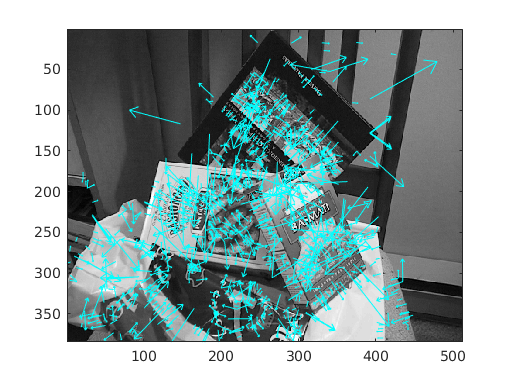
\includegraphics[width=.7\textwidth]{keypoints.png}
 \caption{Found keypoints in `scene.pgm' using SIFT.}
 \label{fig1}
\end{figure}



\begin{appendices}
\section{Code}
 %\lstinputlisting[caption={circorr},label={code:1a}]{../code/circorr.m}
\end{appendices}
\end{document}
